\documentclass[11pt]{article}

\usepackage[a4paper]{geometry}
\geometry{left=2.0cm,right=2.0cm,top=2.5cm,bottom=2.5cm}

\usepackage{ctex} % 支持中文的LaTeX宏包
\usepackage{amsmath,amsfonts,graphicx,subfigure,amssymb,bm,amsthm,mathrsfs,mathtools,breqn} % 数学公式和符号的宏包集合
\usepackage{algorithm,algorithmicx} % 算法和伪代码的宏包
\usepackage[noend]{algpseudocode} % 算法和伪代码的宏包
\usepackage{fancyhdr} % 自定义页眉页脚的宏包
\usepackage[framemethod=TikZ]{mdframed} % 创建带边框的框架的宏包
\usepackage{fontspec} % 字体设置的宏包
\usepackage{adjustbox} % 调整盒子大小的宏包
\usepackage{fontsize} % 设置字体大小的宏包
\usepackage{tikz,xcolor} % 绘制图形和使用颜色的宏包
\usepackage{multicol} % 多栏排版的宏包
\usepackage{multirow} % 表格中合并单元格的宏包
\usepackage{pdfpages} % 插入PDF文件的宏包
\RequirePackage{listings} % 在文档中插入源代码的宏包
\RequirePackage{xcolor} % 定义和使用颜色的宏包
\usepackage{wrapfig} % 文字绕排图片的宏包
\usepackage{bigstrut,multirow,rotating} % 支持在表格中使用特殊命令的宏包
\usepackage{booktabs} % 创建美观的表格的宏包
\usepackage{circuitikz} % 绘制电路图的宏包

\definecolor{dkgreen}{rgb}{0,0.6,0}
\definecolor{gray}{rgb}{0.5,0.5,0.5}
\definecolor{mauve}{rgb}{0.58,0,0.82}
\lstset{
  frame=tb,
  aboveskip=3mm,
  belowskip=3mm,
  showstringspaces=false,
  columns=flexible,
  framerule=1pt,
  rulecolor=\color{gray!35},
  backgroundcolor=\color{gray!5},
  basicstyle={\small\ttfamily},
  numbers=none,
  numberstyle=\tiny\color{gray},
  keywordstyle=\color{blue},
  commentstyle=\color{dkgreen},
  stringstyle=\color{mauve},
  breaklines=true,
  breakatwhitespace=true,
  tabsize=3,
}

% 轻松引用, 可以用\cref{}指令直接引用, 自动加前缀. 
% 例: 图片label为fig:1
% \cref{fig:1} => Figure.1
% \ref{fig:1}  => 1
\usepackage[capitalize]{cleveref}
% \crefname{section}{Sec.}{Secs.}
\Crefname{section}{Section}{Sections}
\Crefname{table}{Table}{Tables}
\crefname{table}{Table.}{Tabs.}

\setmainfont{Palatino_Linotype}[
  Path = ../Fonts/,
  Extension = .ttf
]
\setCJKmainfont{SimHei}[
  Path = ../Fonts/,
  Extension = .ttf
]
\punctstyle{kaiming}
% 偏好的几个字体, 可以根据需要自行加入字体ttf文件并调用

\renewcommand{\emph}[1]{\begin{kaishu}#1\end{kaishu}}

%改这里可以修改实验报告表头的信息
\newcommand{\studentNum}{00000000}
\newcommand{\name}{我是谁}
\newcommand{\exDate}{2025.03.04}
\newcommand{\weekDay}{二}
\newcommand{\ap}{下午}
%%%%%%%%%%%%%%%%%%%%%%%%%%%

\begin{document}

%若需在页眉部分加入内容, 可以在这里输入
% \pagestyle{fancy}
% \lhead{\kaishu 测试}
% \chead{}
% \rhead{}

\begin{center}
    \LARGE \bf 《\, 基\, 础\, 物\, 理\, 实\, 验\, 》\, 实\, 验\, 报\, 告
\end{center}

\begin{center}
    \emph{学号}\underline{\makebox[6em][c]{\studentNum}}
    \emph{姓名}\underline{\makebox[6em][c]{\name}} 
    \emph{实验日期} \underline{\makebox[8em][c]{\exDate}}
    \emph{星期} \underline{\makebox[2em][c]{\weekDay}}\;\underline{\makebox[3em][c]{\ap}}
    {\noindent}
    \rule[8pt]{17cm}{0.2em}
\end{center}

\begin{center}
    \Large \bf 时间测量中随机误差的分布规律
\end{center}

\section*{一、实验目的}

\begin{enumerate}
    \item 认识多次重复等精度测量过程中随机误差的离散性和分布规律
    \item 学习直接测量量的不确定度计算和表示方法。
\end{enumerate}

\section*{二、实验原理}

本实验使用秒表重复测量电子节拍器的周期$ T_0 $,测量结果记为$ T_1, T_2, \cdots, T_n $。如果测量次数足够多,那么测量结果处于$ T $附近的概率密度趋近于正态分布
$$
p(T)=\dfrac{1}{\sigma\sqrt{2\pi}}exp\left[-\dfrac{\left(T-\overline{T}\right)^2}{2\sigma^2}\right]
$$
其中, $\overline{T}=\dfrac{1}{n}\sum_{j=1}^nT_j$ 表示周期测量值的平均值, $\sigma=\sqrt{\dfrac{\sum_{j=1}^n\left(T_j-\overline{T}\right)^2}{(n-1)}}$ 表示周期测量值的标准差。

正态分布理论表明,测量结果处于置信区间 $\left[\overline{T}-\sigma, \overline{T}+\sigma\right]$ , $\left[\overline{T}-2\sigma, \overline{T}+2\sigma\right]$ 和 $\left[\overline{T}-3\sigma, \overline{T}+3\sigma\right]$内的置信概率 $P$ 分别为
$$
\int_{\overline{T} - \sigma}^{\overline{T} + \sigma}p(T)dT=0.683
$$
$$
\int_{\overline{T} - 2\sigma}^{\overline{T} + 2\sigma}p(T)dT=0.954
$$
$$
\int_{\overline{T} - 3\sigma}^{\overline{T} + 3\sigma}p(T)dT=0.997
$$

基于标准差,可以计算周期测量的$A$类标准不确定度
$$
u_A=\dfrac{\sigma}{\sqrt{n}}
$$
本次实验中,周期测量的$B$类标准不确定度主要来自实验者的估计误差(反应
时间)$\Delta_{\text{估}}$和秒表的仪器误差$\Delta_{\text{仪}}$
$$
u_B=\dfrac{\sqrt{\Delta_{\text{估}}^2+\Delta_{\text{仪}}^2}}{C}\quad\text{(其中, }C\text{为置信系数)}
$$
两类不确定度的合成和扩展公式为
$$
u_p=\sqrt{(t_pu_A)^2+(k_pu_B)^2}\quad\text{(其中}k_p\text{和}t_p\text{分别为置信因子和}t\text{因子)}
$$

最后,节拍器周期测量结果表示为
$$
T=\overline{T}\pm u_p\quad P=0.95
$$

\section*{三、实验仪器}

电子节拍器,秒表

\section*{四、实验内容}

\begin{enumerate}
    \item 用秒表测量电子节拍器周期,测量$n$组数据, $n=200$。
    \item 计算测量结果的平均值$\overline{T}$和标准差$\sigma$。
    \item 根据测量结果的离散程度和极限差$R=T_{max}-T_{min}$,合理设置小区间步长$\Delta T$和个数$K$。
    \item 统计区间$\left[T_i-\dfrac{\Delta T}{2}, T_i+\dfrac{\Delta T}{2}\right]$内的频率$n_i$(数据点个数)、概率$P_i$($\dfrac{n_i}{n}$)和概率密度$p_i$($\dfrac{P_i}{\Delta T}$),并绘制$p_i$随区间中值$T_i$变化的直方图。
    \item 计算正态分布函数$p(T)=\dfrac{1}{\sigma\sqrt{2\pi}}exp\left[-\dfrac{\left(T-\overline{T}\right)^2}{2\sigma^2}\right]$在各中值$T_i$位置的函数值。
    \item 在$p_i$\,-\,$T_i$直方图上添加$p(T_i)$\,-\,$T_i$散点图,检验测量结果是否符合正态分布。
    \item 分别统计测量结果出现在置信区间 $\left[\overline{T}-\sigma, \overline{T}+\sigma\right]$ , $\left[\overline{T}-2\sigma, \overline{T}+2\sigma\right]$ 和 $\left[\overline{T}-3\sigma, \overline{T}+3\sigma\right]$ 内的概率$P$,并与理论值比较。
    \item 计算测量结果的$A$类标准不确定度和$B$类标准不确定度,并写出置信概率为$P=0.95$时的测量结果完整表达式。
\end{enumerate}

\section*{五、数据记录}

用秒表测电子节拍器周期,记录200组数据。原始数据见数据记录表。

\section*{六、数据处理}

\begin{enumerate}
    \item 测量结果的平均值$\overline{T}$和标准差$\sigma$,$T$的最大值为$T_{max}$,最小值为$T_{min}$,得到以下数据(见表1)
    \begin{figure}[H]
        \centering
        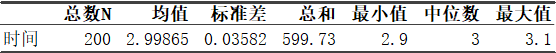
\includegraphics[width=15cm]{Fig/Table1.png}\\
        \small{表1}
    \end{figure}
    \item 合理设置小区间步长和个数 $\Delta T=0.05s; k=8$
    \item 统计区间内的频数$n_i$,概率$\dfrac{n_i}{n}$,概率密度$\dfrac{n_i}{n\Delta T}$,详见表2,并绘制频数随区间中值变化直方图(图1)和概率密度随区间中值变化直方图(图2)。
    \begin{figure}[H]
        \centering
        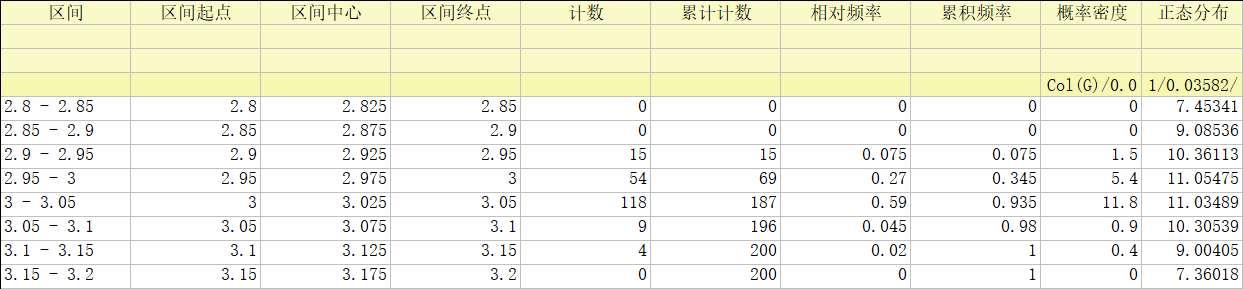
\includegraphics[width=15cm]{Fig/Table2.png}\\
        \small{表2}
    \end{figure}
    \begin{figure}[H]
    \centering
    \subfigure[图1]{
        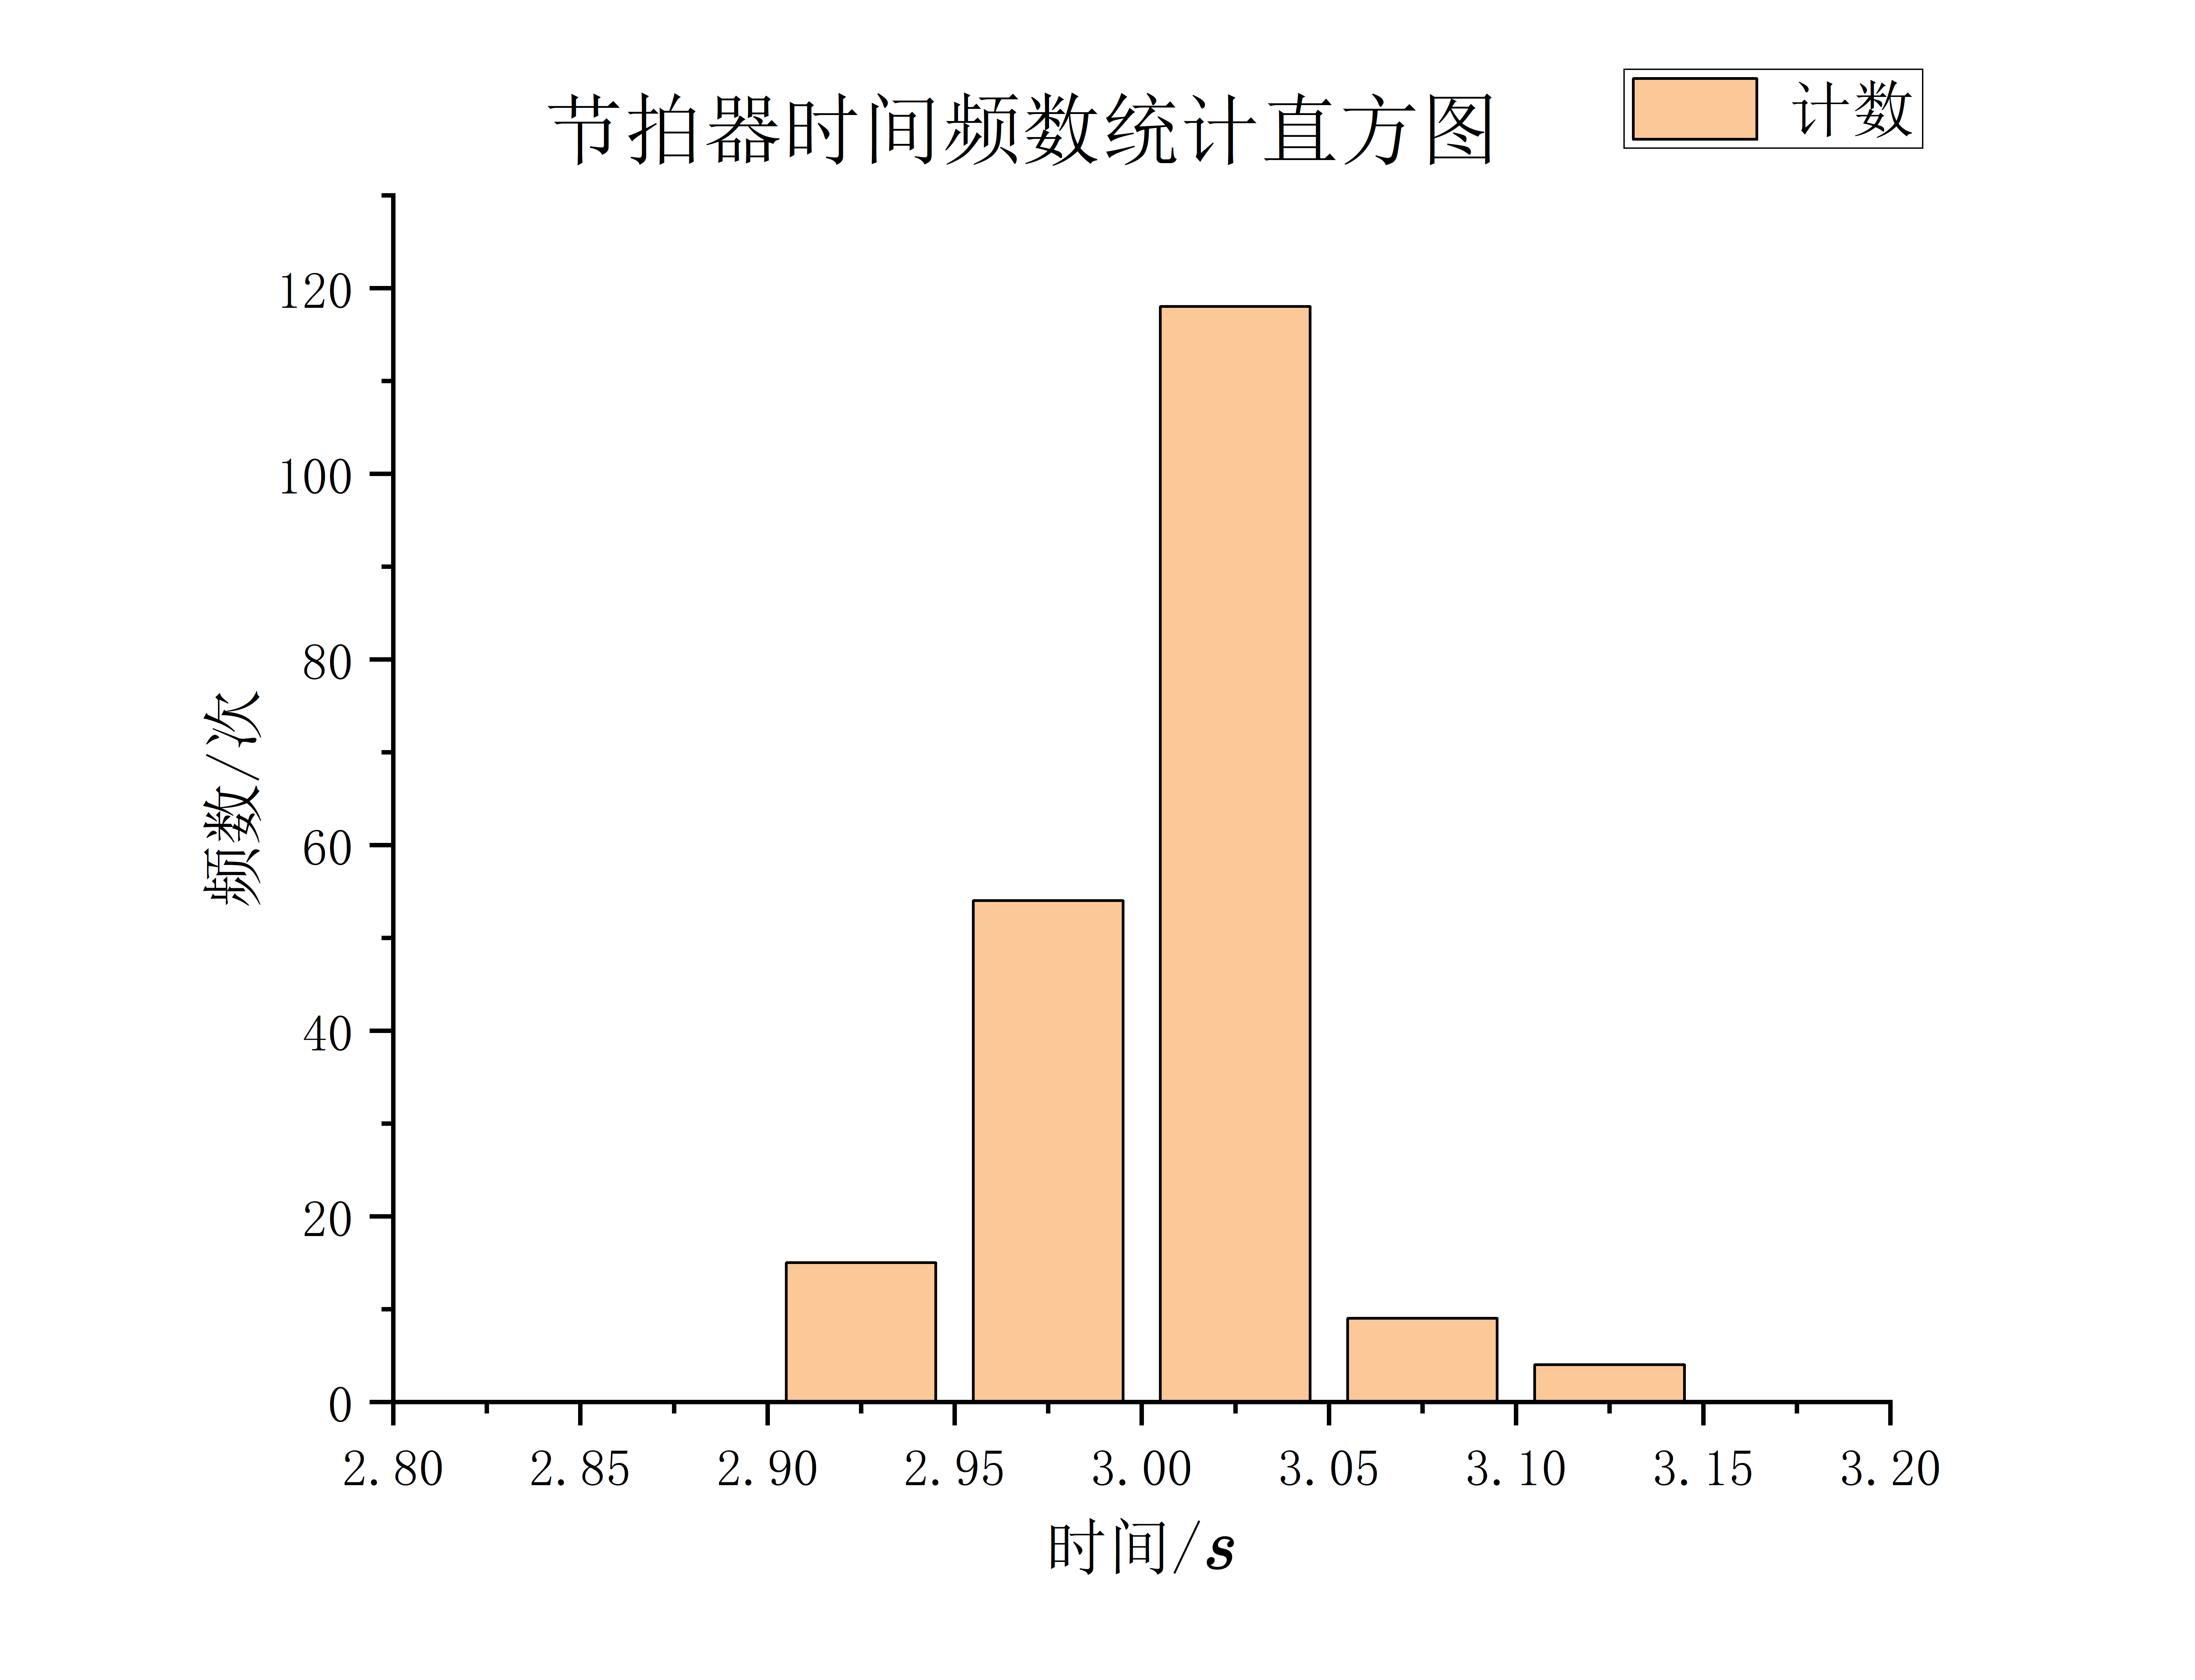
\includegraphics[width=7.5cm]{Fig/Graph1.png}}
    \hspace{0.5in}
    \subfigure[图2]{
        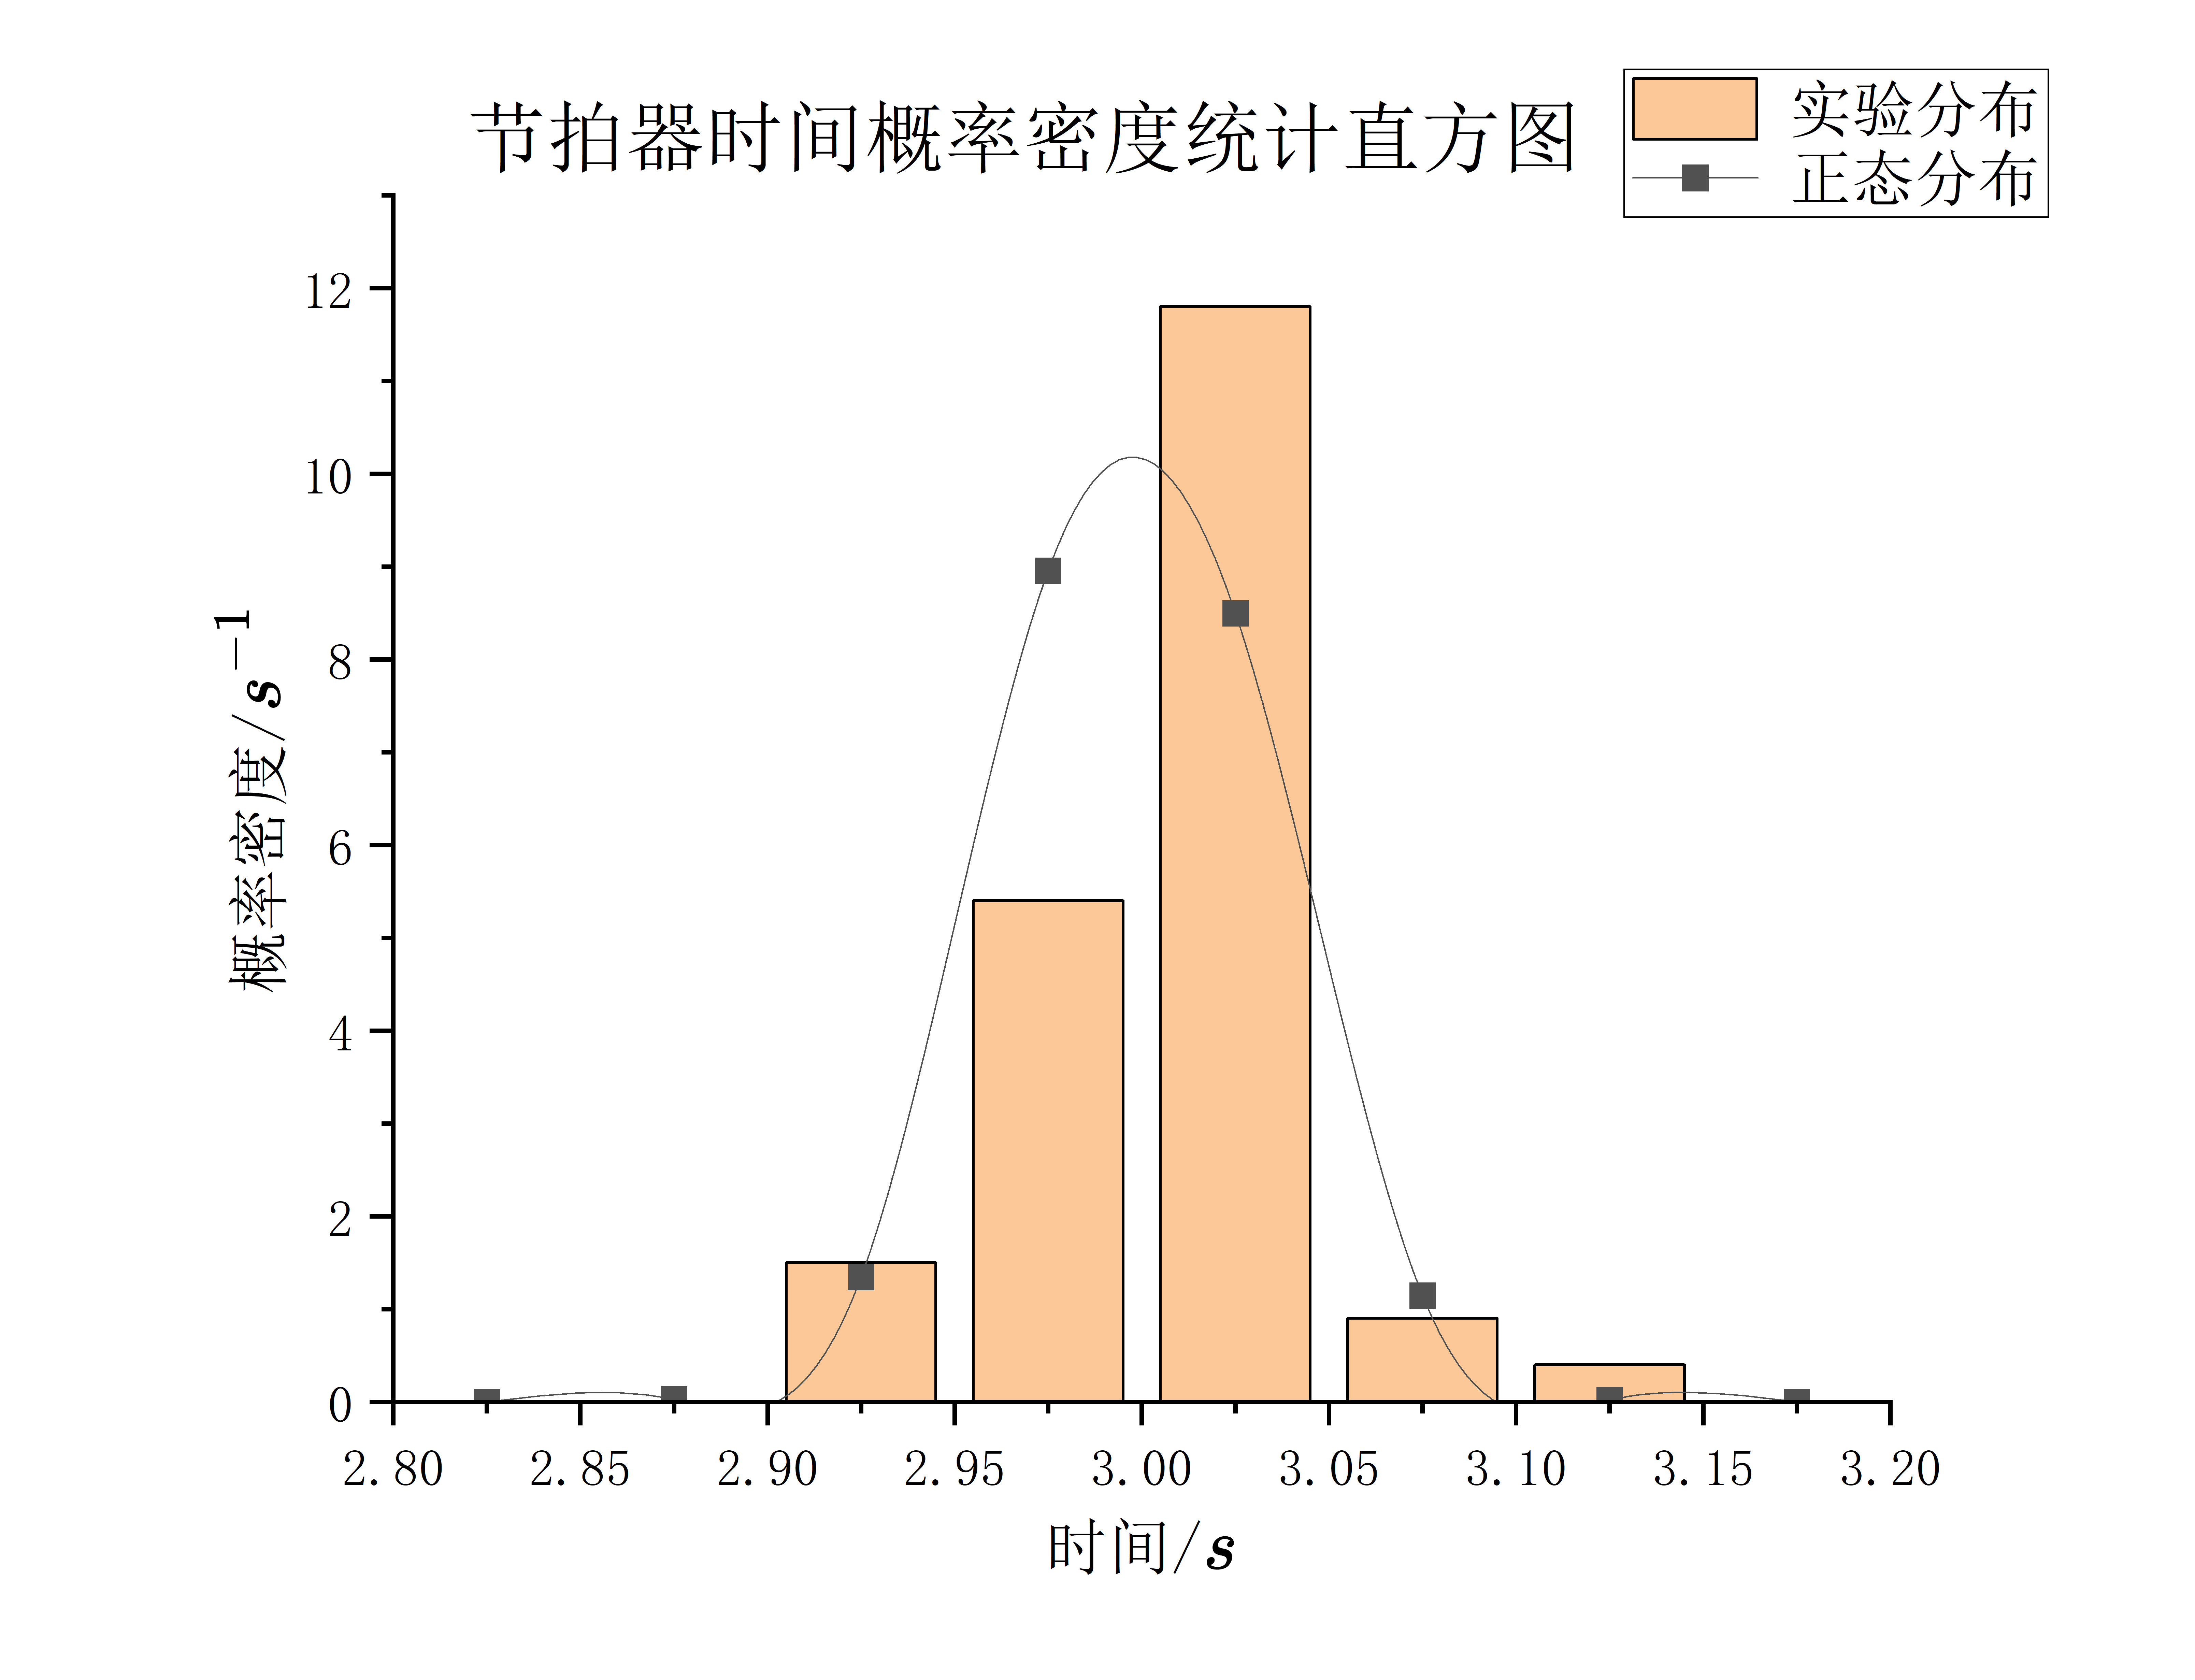
\includegraphics[width=7.5cm]{Fig/Graph2.png}}
    \hspace{0.5in}
    \end{figure}
    \item 计算正态分布函数在各中值位置的函数值$f(T)=\dfrac{1}{\sigma\sqrt{2\pi}}exp\left[-\dfrac{\left(T-\overline{T}\right)^2}{2\sigma^2}\right]$,并添加点线图,检验是否符合正态分布。(见图2)
    \item 统计测量结果出现在置信区间内的概率,并与理论值比较。
    $$
    p(\sigma)=\int_{\overline{T}-\sigma}^{\overline{T}+\sigma}f(T)dT=0.745\quad\text{理论值为}0.683
    $$
    $$
    p(2\sigma)=\int_{\overline{T}-2\sigma}^{\overline{T}+2\sigma}f(T)dT=0.965\quad\text{理论值为}0.954
    $$
    $$
    p(3\sigma)=\int_{\overline{T}-3\sigma}^{\overline{T}+3\sigma}f(T)dT=1.000\quad\text{理论值为}0.997
    $$
    \item 计算不确定度
    $A$类不确定度:$u_A=\dfrac{\sigma}{\sqrt{n}}=0.00253s$
    $B$类不确定度:$u_B=\dfrac{\sqrt{\Delta_{\text{估}}^2+\Delta_{\text{仪}}^2}}{C}=\dfrac{\sqrt{0.2^2+0.01^2}}{3}=0.06675s$
    合成不确定度:$u_p=\sqrt{(t_pu_A)^2+(k_pu_B)^2}=\sqrt{(1.96\cdot0.00253)^2+(1.96\cdot0.06675)^2}=0.06427s$
    \item 测量结果的完整表达式为:$T=(2.99865\pm0.06427)s\quad(P=0.95)$
\end{enumerate}

\section*{七、误差分析}

\begin{enumerate}
    \item 实验人员反应延迟不稳定
    \item 实验人员注意力涣散
    \item 电子节拍器的仪器误差
    \item 秒表的仪器误差
\end{enumerate}

\section*{八、思考题}

\begin{enumerate}
    
    \item 若测量结果偏离正态分布,请分析其主要原因。
    
    答:仪器测量结果有误差;实验人员反应时间不固定;实验人员在长时间实验中易注意力涣散;实验仪器的精度不够小导致出现不少值位于区间端点,例如测得大量$3.00s$导致处于$[3.00,3.05)$的频数大于处于$[2.95,3.00)$的频数。
    
    \item 在不考虑系统误差的前提下,多次等精度测量的随机误差分布有哪些特征?

    答:随机误差基本服从以$0$为平均值的正态分布。

\end{enumerate}

\section*{九、实验结论}

本实验使用秒表重复测量电子节拍器的周期$T_i$,并且使用统计学方法求得周期$T$。该实验中的随机误差与正态分布有一定不吻合,但总体呈现基本符合正态分布。
经过$200$次测量,测得电子节拍器的周期为
$$
T=(2.99865\pm0.06427)s\quad(P=0.95)
$$

\end{document}